\documentclass[12pt]{article}
\usepackage{tgtermes}
\usepackage[english]{babel}
\usepackage[utf8]{inputenc}
\setlength{\paperwidth}{21cm}   % A4
\setlength{\paperheight}{29.7cm}% A4
\setlength\topmargin{-0.5cm}    
\setlength\oddsidemargin{0cm}   
\setlength\textheight{24.7cm} 
\setlength\textwidth{16.0cm}
\setlength\columnsep{0.6cm}  
\newlength\titlebox 
\setlength\titlebox{5cm}
\setlength\headheight{5pt}   
\setlength\headsep{0pt}
\pagestyle{plain}
\usepackage{color}
\usepackage[natbibapa]{apacite}
\usepackage{xurl}
\usepackage[colorlinks,citecolor=blue,urlcolor=blue, linkcolor=blue, bookmarks=false,hypertexnames=true]{hyperref}
\usepackage{url}
%\usepackage{libertine}
\usepackage{float}
\usepackage{graphicx}
\usepackage{amsmath}
\usepackage{doi} % hyperlink URLs
\renewcommand{\doi}{DOI:~}
\renewcommand{\baselinestretch}{1.25}

\title{Google PageRank}

\date{Nov 30, 2022}

\begin{document}

\maketitle

\begin{abstract} 
\noindent In this paper we introduce the Google PageRank model and the commonly used ideas for computation, especially iteration method that has been adopted to efficiently compute the PageRank result. There is also related information of the computation process including the computation cost, rate of convergence, acceleration techniques, etc. Given that there are billions of webpages on Google that need to be ranked, we will also explore how matrices of this scale are stored by replicating its idea through storing sparse matrices in Matlab. In the end, we also have a section that introduces current research on quantum PageRank algorithm .  \end{abstract}

\tableofcontents
\section{Introduction}

\paragraph{} Google is well known to be an effective search engine, and a major factor that contributes to its success is the PageRank algorithm developed by Google’s founders, Larry Page and Sergey Brin, when they were graduate students at Stanford University[1]. PageRank is determined entirely by the link structure of the World Wide Web. It is recomputed about once a month and does not involve the actual content of any Web pages or individual queries. Then, for any particular query, Google finds the pages on the Web that match that query and lists those pages in the order of their PageRank.

\paragraph{} In real life, Google operates on a scale that is more than 10 billion * 10 billion web pages. Therefore, it is crucial for Google to adopt an effective method of computing pagerank and display the most relevant results to their users. The result of PageRank is highly related to the concept of computing eigenvalues and eigenvectors, and things will undoubtedly be complicated when there is an enormous webpage matrix to process. We need the “dominant eigenvector” of the matrix that contains the information of the PageRank result, and we learn how pages are ordered within that resulting vector.

\paragraph{} In order to compute the dominant vector, we will introduce the power iteration method of computing the eigenvector, as well as its related information including computation cost, memory storage, asymptotic complexity, etc. To emulate the storage of web page information, we also introduce the sparse matrix representation and calculate the conditions that guarantee a fast rate of convergence.

\section{PageRank Matrix}
\paragraph{} The PageRank algorithm performs calculation on a PageRank matrix. Given a web page, the basic idea might be to look at how many pages are linking to this page. In terms of graph theory, what actually matters is the in and out degree of "vertices", which represent web pages. 

\subsection{Markov Model behind PageRank}
\paragraph{} Markov Chain helps in predicting the behavior of the system which is in transition from one state to another by considering only the current state[11]. The idea of Markov chain is part of the broad idea of constructing PageRank matrix, since "ranking pages" is essentially similar to determine which pages are more likely to be the "next page" for the current page.

\subsection{PageRank Matrix Example}
We can show how a PageRank matrix is constructed by an example of "simple web".\\
\begin{center}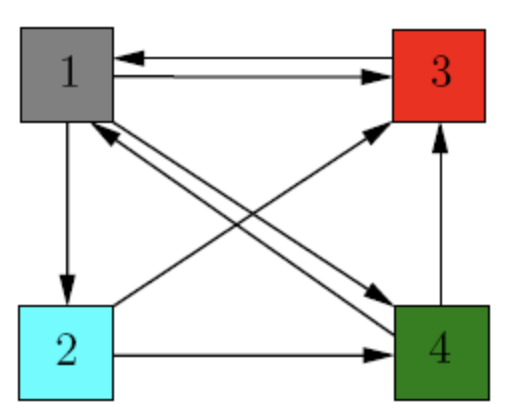
\includegraphics[]{images/simple_web.png}\end{center}\\
Based on in and out degrees of vertices, this graph corresponds to PageRank Matrix:\begin{center}
$
\begin{bmatrix}
0 & 0 & 1 & 1/2\\
1/3 & 0 & 0 & 0\\
1/3 & 1/2 & 0 & 1/2\\
1/3 & 1/2 & 0 & 0
\end{bmatrix}
$\\
\end{center}
If we want to assign an additional weight $0.85$ to the matrix (meaning 0.85 chance that the next web page exactly follows the above matrix), the PageRank matrix becomes: \begin{center}
(0.15/4) * $
\begin{bmatrix}
1 & 1 & 1 & 1\\
1 & 1 & 1 & 1\\
1 & 1 & 1 & 1\\
1 & 1 & 1 & 1
\end{bmatrix}
$  + 0.85 * $
\begin{bmatrix}
0 & 0 & 1 & 1/2\\
1/3 & 0 & 0 & 0\\
1/3 & 1/2 & 0 & 1/2\\
1/3 & 1/2 & 0 & 0
\end{bmatrix}
$
\end{center}
Note that the PageRanks form a probability distribution over web pages, so the sum of all web pages’ PageRanks will be one[10]. After obtaining the matrix, we need an efficient way of calculating PageRank vector, which is the dominant eigenvector that corresponds to an eigenvalue whose magnitude is greater than all other eigenvalues of the PageRank matrix.\\



\subsection{Ideas of Computing PageRank Vector}

\paragraph{} In this section, we want to explore a few ideas of computing the PageRank eigenvector[5]:

\begin{itemize}
    \item[1.] From a dynamical system point of view:
\paragraph{} Assume that initially the importance is uniformly distributed among these four web pages, so each part is 1/4. Let us denote this initial rank vector as v. Each incoming link increases the page's importance, so we update each page's rank by adding the incoming link's importance to the current value. We iterate this process.

\paragraph{}$A = \begin{bmatrix}
0 & 0 & 1 & 1/2\\
1/3 & 0 & 0 & 0\\
1/3 & 1/2 & 0 & 1/2\\
1/3 & 1/2 & 0 & 0
\end{bmatrix}
, v = \begin{bmatrix}0.25 \\0.25 \\0.25 \\0.25 \\\end{bmatrix}$
\paragraph{} $Av = \begin{bmatrix}0.37 \\0.08 \\0.33 \\0.20 \\\end{bmatrix},  A^2v = A(Av) = \begin{bmatrix}0.43 \\0.12 \\0.27 \\0.16 \\\end{bmatrix}, A^3v = \begin{bmatrix}0.35 \\0.14 \\0.29 \\0.20 \\\end{bmatrix},  ...$
\paragraph{} After several iterations, $A^kv$ tends to the equilibrium value: $\begin{bmatrix}0.38 \\0.12 \\0.29 \\0.19 \\\end{bmatrix}$ So this is the PageRank vector of our web graph.

    \item[2.] From linear algebra point of view: 
    \paragraph{}Let us consider the matrix A as an equation system. Denote the four nodes as $c_1, c_2, c_3, c_4$. So we get:

\begin{equation*}
  \left\{
    \begin{aligned}
      & c_1 = 1 * c_3 + \frac{1}{2} * c_4 \\
      & c_2 = \frac{1}{3} * c_1 \\
      & c_3 = \frac{1}{3} * c_1 + \frac{1}{2} * c_2 + \frac{1}{2} * c_4 \\
      & c_4 = \frac{1}{3} * c_1 + \frac{1}{2} * c_2 \\
    \end{aligned}
  \right.
\end{equation*}

\paragraph{}This equation system actually solves $Ac = c$. By calculation, we get $\frac{1}{31}\begin{bmatrix}12 \\4 \\9 \\6 \\\end{bmatrix} \approx \begin{bmatrix}0.38 \\0.12 \\0.29 \\0.19 \\\end{bmatrix}$. 
\paragraph{}This is the eigenvector of this matrix. We got this result because PageRank only reflects the relative importance of the four nodes. Since the eigenvector indices are scalar multiples of each other, by solving this system of equations we obtain our PageRank vector.
    \item[3.] From the probabilistic point of view:
\paragraph{}The importance of a web page is measured by how popular it is, in terms of how many incoming links it gets. Therefore, when we construct the matrix, we are actually estimating the probability of users visiting different web pages. So some pages are marked with $\frac{1}{2}$ probability and some with $\frac{1}{3}$ probability.
\paragraph{}From this point of view, the initial probability is distributed equally, so $\begin{bmatrix}\frac{1}{4} \\\frac{1}{4} \\\frac{1}{4} \\\frac{1}{4} \\\end{bmatrix}$. For each step k, we have $A^k*v$ probability of being visited. When the vector stabilizes, we can get our PageRank vector: $\begin{bmatrix}0.38 \\0.12 \\0.29 \\0.19 \\\end{bmatrix}$.
    
\end{itemize}

\paragraph{} We can understand that PageRank Ranking can be calculated by iteration. In the next section, we will introduce the Power Iteration Method, which is something that we can actually use to compute the dominant eigenvector in real life, and it illustrates how iteration works in detail.



\section{Power Iteration Method}

\paragraph{}When calculating Google Page Ranking, what we are most concerned about is to obtain the dominant eigenvector, so as to rank Google pages. The Power Iteration method is a very simple way to extract the largest eigenvalue. The algorithm is also known as the Von Mises iteration. 

\subsection{Algorithm}

\paragraph{}let A be an $m * m$ diagonalizable matrix, A dominant eigenvalue of A is an eigenvalue $\lambda_1$ whose magnitude is greater than all other eigenvalues of A  with $|\lambda_1|>|\lambda_2|>|\lambda_3|>...>|\lambda_n|$ for all $i=2,3,...,n$. If it exists, an eigenvector $v_1$ associated to $\lambda_1$ is called a dominant eigenvector.

\paragraph{}The iteration is[6]:

\begin{itemize}
    \item[1.] For the given matrix A, we random form an vector $v_0$ and let $i = 1$
    \item[2.] let $u_{i-1} = \frac{v_{i-1}}{||v_{i-1}||_2}$
    \item[3.] let $v_i = Au_{i-1}$
    \item[4.] $\lambda_i = u_{i-1}^TAu_{i-1}$
    \item[5.] $i = i+1$
    \item[6.] Repeat steps (2) to (5) until proper convergence is found, return $u_i = \frac{v_i}{||v_i||_2}$.
\end{itemize}

\subsection{Example}

\paragraph{}let A be the matrix, $A = \begin{bmatrix}1 & 3 \\2 & 2 \\\end{bmatrix}$ has a dominant eigenvalue. Let us observe the result of multiplying the matrix A times a "random" vector, say $x_0 = \begin{bmatrix}-5 \\5 \\\end{bmatrix}$, use the iteration above[6]:\\


\begin{itemize}
    \item[] $x_1 = Ax_0 = \begin{bmatrix}1 & 3 \\2 & 2 \\\end{bmatrix}\begin{bmatrix}-5 \\5 \\\end{bmatrix} = \begin{bmatrix}10 \\0 \\\end{bmatrix}$
    \item[] $x_2 = A^2x_0 = \begin{bmatrix}1 & 3 \\2 & 2 \\\end{bmatrix}\begin{bmatrix}10 \\0 \\\end{bmatrix} = \begin{bmatrix}10 \\20 \\\end{bmatrix}$
    \item[] $x_3 = A^3x_0 = \begin{bmatrix}1 & 3 \\2 & 2 \\\end{bmatrix}\begin{bmatrix}10 \\20 \\\end{bmatrix} = \begin{bmatrix}70 \\60 \\\end{bmatrix}$
    \item[] $x_4 = A^4x_0 = \begin{bmatrix}1 & 3 \\2 & 2 \\\end{bmatrix}\begin{bmatrix}70 \\60 \\\end{bmatrix} = \begin{bmatrix}250 \\260 \\\end{bmatrix} = 260\begin{bmatrix}\frac{25}{26} \\1 \\\end{bmatrix}$
\end{itemize}




\paragraph{}Multiplying $x_0$ repeatedly by the matrix A has resulted in moving the vector very close to the dominant eigenvector of A, so our vector approaches $\begin{bmatrix}1\\1 \\\end{bmatrix}$, which is the dominant eigenvector of the system.

\subsection{Convergence of the Power Iteration Method}
\paragraph{}Let $v_1, v_2,..., v_n$ be the eigenvectors that form a basis of $R^n$, with corresponding eigenvalues $\lambda_1, \lambda_2, ..., \lambda_n$, and $|\lambda_1|>|\lambda_2|>|\lambda_3|>...>|\lambda_n|$ for all $i=2,3,...,n$. Express the initial vector in the basis as $x_0 = a_1v_1 + a_2v_2+ ... +a_nv_n$, assume $a_1\neq0$, construct a sequence of vectors from this $x_k = Ax_k-1$, when $k=1,2,3...$, so we get:
\paragraph{} $x_1 = Ax_0 = a_1Av_1 + a_2Av_2 + ... + a_nAv_n = a_1\lambda_1v_1 + a_2\lambda_2v_2+...+a_n\lambda_nv_n$
\paragraph{} $x_2 = A^2x_0 = a_1\lambda_1Av_1 + a_2\lambda_2Av_2+...+a_n\lambda_nAv_n = a_1\lambda_1^2v_1 + a_2\lambda_2^2v_2+...+a_n\lambda_n^2v_n$

\paragraph{}get vector sequence:
\paragraph{}$x_1 =Ax_0 = a_1\lambda_1v_1 + a_2\lambda_2v_2+...+a_n\lambda_nv_n$
\paragraph{}$x_2 =A^2x_0= a_1\lambda_1^2v_1 + a_2\lambda_2^2v_2+...+a_n\lambda_n^2v_n$
\paragraph{}...
\paragraph{}$x_k =A^kx_0 = a_1\lambda_1^kv_1 + a_2\lambda_2^kv_2+...+a_n\lambda_n^kv_n$

\paragraph{}Then, $A^kx_0 = a_1\lambda_1^kv_1 + a_2\lambda_2^kv_2+...+a_n\lambda_n^kv_n = \lambda_1^k[a_1v_1+a_2(\frac{\lambda_2}{\lambda_1})^kv_2+...+a_n(\frac{\lambda_n}{\lambda_1})^kv_n]$

\paragraph{}Since $\lambda_1$ is the dominant eigenvalue, so when $k\rightarrow\infty$, $(\frac{\lambda_i}{\lambda_1})^k\rightarrow0$, so $A^kx_0 \approx \lambda_1^ka_1v_1$

\paragraph{}From the above results, it also can be seen that: when $k\rightarrow\infty$, $A^kx_0 \approx \lambda_1^ka_1v_1$ and $A^{k+1}x_0 \approx \lambda_1^{k+1}a_1v_1$, we get: $\lambda_1 \approx \frac{(A^{k+1}x_0)}{(A^kx_0)}$.


\subsubsection{Overflow Problem}
\paragraph{}When $|\lambda_1| > 1$, the nonzero component in $x_k$ will tend to be $\infty$ as $k\rightarrow\infty$, which may cause overflow during computer calculation. Also when $|\lambda_1| < 1$, the nonzero component in $x_k$ will tend to be $0$ as $k\rightarrow\infty$.
\paragraph{}In actual calculation, in order to avoid the calculation process of the case where the absolute value is too large or too small, usually the vector is "normalized" in each iteration step.

\subsubsection{Convergence Failed}
\paragraph{}As we see above, the convergence (if existent) is determined by $\frac{|\lambda_2|}{|\lambda_1|}$. If the value of the next dominant eigenvalue is close to the current dominant eigenvalue, the iteration will converge slowly. When $\lambda_2 = \lambda_1$ or $|\lambda_2| = |\lambda_1| (\lambda_2 \neq \lambda_1)$, the converge will fail[7].


\subsection{Pseudo-code}
\begin{verbatim}
function [lam, u] = rqi(A,x,k)
for j = 1:k
    u=x/norm(x);
    x=A*u;
    lam=u'*x;
 end
 u=x/norm(x);[6]
\end{verbatim}


\subsection{The advantage and disadvantage of Power Iteration Method}
\paragraph{} When calculating PageRake vectors, it is usually understood as an eigenvector problem, especially as finding the dominant eigenvector. There are many ways to find the dominant eigenvector, but we use Power Iteration more because it has the following benefits:
\begin{itemize}
    \item Consider iterates of the power method applied to a completely dense matrix, it can in its most naive form only compute $\lambda_1$ and ignore $\lambda_2,...,\lambda_n$, thus saving computer memory space and making computing more efficient.
    \item Power iteration is very simple algorithm, so it is easy to implement. The most time-consuming part of the algorithm is the matrix-vector multiplication, so for very large sparse matrices such as the PageRank Matrix, it is efficient with a proper implementation (such as by exploiting its nature of being sparse).
\end{itemize}

\paragraph{} The disadvantage of the power method is also obvious: it depends on the rate of convergence, it might be slow. In the next section we will discuss the two techniques of acceleration.

\subsection{Acceleration Techniques for the PageRank Power Iteration Method}
\paragraph{}Solving PageRank using power method may seem like a simple problem, but in reality, this matrix is called "the world's largest matrix computation", so it presents huge computational and memory challenges. Although Power Iteration seems to be a classic calculation method that can quickly calculate the results, its calculation is still not fast enough in the face of such a huge matrix. The size and sparsity of the matrix limit the solution method. Iterations are very expensive. Some researchers have investigated ways to speed up the computation of the solution, in order to reduce the computation time and the amount of work per iteration. Here are two ways to speed up power method calculations[8]:
\begin{itemize}
    \item[1.] Adaptive PageRank. Some researchers have noticed that some pages converge to their PageRank values faster than others. Because of the approach they take: Converge with the elements of the PageRank vector, lock in those values that converge faster, and don't use them in subsequent calculations. After research, this approach provided a small 17\% speedup in the calculation of PageRank.
    \item[2.] Partitions the web into dangling and non-dangling nodes. Some researchers divide the web into dangling nodes and non-dangling nodes and partition and aggregate them separately. Since Google's fix for dangling nodes produces a block of the same row, a centrally aggregated block can be solved precisely and efficiently. In such cases, the m*m problem in the algorithm can be reduced to several much smaller k*k matrix problems, where k is the number of non-dangling nodes on the web. If $k = \frac{1}{s}n$, then the time until convergence is reduced by a factor of s over the power method.
\end{itemize}


\section{Store PageRank Matrices}
\paragraph{} It is intuitively not possible for Google to store billions of webpages in a single matrix; instead, according to Google's research paper, the most up-to-date solution for storage is called Bigtable[4], which is a distributed storage system for structured data. PageRank matrices are also stored by using these sparse data structure under distributed databases. Since a page is only linked to a finite amount of other pages, a supposedly "full-size" PageRank matrix that models the Internet will contain an enormous amount of zero's. Therefore, the usage of sparse data structure makes perfect sense for today's Internet.


\subsection{Store Sparse Matrices in Matlab}
\paragraph{} We cannot cover all details of how Google stores their PageRank thoroughly within the range of this paper, but the idea of efficiently storing PageRank matrices is worth exploring. If we ever need to implement PageRank algorithm to sort out a certain amount of web pages, it would be very helpful if there is an efficient way that requires less space to store matrices, so the cost of computation is lowered, and the speed of computation should be noticeably improved.

\paragraph{} Since Matlab is a commonly used tool for mathematical computation, it is helpful for us to learn about storing sparse matrices in Matlab, and how we can use sparse matrices for eigenvector computation.

\subsection{Properties of Sparse Matrices}
\paragraph{} Sparse matrices provide an efficient method of storing double or logical data that has a large percentage of zeros[2]. While full (or dense) matrices store every single element in memory regardless of value, sparse matrices store only the nonzero elements and their row indices. For this reason, using sparse matrices can significantly reduce the amount of memory required for data storage.

\paragraph{} According to the official document of Matlab, by default the command $sparse()$ converts a full matrix into a sparse matrix and store it in double precision. The memory usage of sparse matrices is also significantly reduced compared to that of a full matrix.

\paragraph{} Here is the statistics of storing a sparse matrices in Matlab, let D be the matrix representation of the discrete 5-point Laplacian on a square 64x64 grid with a nested dissection ordering. This is a 4096x4096 matrix with 20224 nonzero entries[3].

\begin{verbatim}
                 Sparse           Full
Memory       0.25 megabyte    128 megabytes
Compute Dx    0.2 seconds      30 seconds
Solve Dx=b     10 seconds      >12 hours
\end{verbatim}

\subsection{Example of Using Sparse matrices}
\textbf{Code}:
\begin{verbatim}
M_full = magic(1100);          % Create a 1100-by-1100 matrix.
M_full(M_full > 50) = 0;       % Set elements > 50 to zero.
M_sparse = sparse(M_full);     % Create sparse matrix of same.
\end{verbatim}

\noindent \textbf{Output}:
\begin{verbatim}
Name             Size                Bytes  Class     Attributes

M_full        1100x1100            9680000  double              
M_sparse      1100x1100               9608  double    sparse  
\end{verbatim}

\noindent As we can see, the storage space is significantly reduced.\\

\subsection{Compute PageRank Using Sparse Matrices}
Here is a simple Matlab example here that shows using sparse matrices will produce the same dominant eigenvector as the original matrix.\\

\noindent\textbf{Code}:
\begin{verbatim}
A = [0,0,1,1/2;0,1/3,0,0;1/2,1/3,0,1/2;1/2,1/3,0,0];
T = 0.85*A+0.15/4*ones(4);
T_sparse = sparse(T);
[V1,D1]=eigs(T,1);
PageRank = V1/sum(V1)
[V2,D2]=eigs(T_sparse,1);
PageRank_sparse = V2/sum(V2)
\end{verbatim}

\noindent\textbf{Output}:
\begin{verbatim}
PageRank =
    0.4042
    0.0523
    0.3194
    0.2241
PageRank_sparse =
    0.4042
    0.0523
    0.3194
    0.2241
\end{verbatim}

\noindent As we can see, sparse representation of the transition matrix will yield the same PageRank result as the original transition matrix, and it is safe to use sparse matrices for more efficient computation.\\


\section{Current Research on PageRank}
\paragraph{} Let's talk about the current research on PageRank, the name of this algorithm is Quantum PageRank Algorithm[9].
\paragraph{} Let $I_c$ is defined as the vector, its entries are the classical importance or PageRanks of every page $P_i$. The definition of the PageRank is:

\begin{equation*}
  I_c(P_i) := \sum_{P_j \in B_i} \frac{I_c(P_j)}{outdeg(P_j)}
\end{equation*}

\paragraph{} where $B_i$ is the set of nodes linked to node Pi, and $outdeg(P_j)$ is the degree out from node $P_j$. This formula means that the importance of a node depends on how many links connect it. The more nodes link to a node, the higher the node's rank will be. At the same time, we also consider that users will walk randomly in different nodes, so the associated connectivity $N*N$ matrix H defined as:


\begin{equation*}
  \left\{
    \begin{aligned}
      & \frac{I_c(P_j)}{outdeg(P_j)}\qquad  if P_j \in B_i,\\
      & 0       \qquad\qquad\qquad otherwise, \\
    \end{aligned}
  \right.
\end{equation*}

\paragraph{} where N is the number of nodes in the network. So we get a random matrix E, whose column sum is 1. We also need to combine it with another matrix \emph{1} to get an original irreducible matrix, expressed by the equation:

\begin{equation*}
  \alpha E + \frac{(1-\alpha)}{N} \emph{1}
\end{equation*}

\paragraph{} According to Brin and Page that the optimal value is $\alpha = 0.85$, This mixing can be interpreted as the user going from one node to another with probability $\alpha$, and randomly jumping to one of the node with probability $1-\alpha$. Finally, we obtain the eigenvectors by converges.

\paragraph{} In recent years, some new algorithms have emerged, such as New Quantum PageRank Algorithm. They improve on the original quantum algorithm, able to break the degeneracy of remaining nodes and detect secondary hubs suppressed by the classical algorithm, achieving more stable results.

\section{Conclusion}
\paragraph{} In this paper, we introduced the general model of PageRank matrix and ideas of computing the PageRank result. Moreover, we introduced the power iteration method in detail, as well as its properties including the rate of convergence, potential errors, and some acceleration techniques and so on. We also discussed how sparse matrices plays an important role in computing PageRank results and demonstrated a few Matlab examples.

\paragraph{} If readers are interested in learning more about PageRank, we included a section that talks about research about the quantum algorithm for PageRank in recent years. Readers can find more details in the reference section.

\begin{thebibliography}{9}
\bibitem{1}
[1] Matlab, \emph{PageRank}\\
\url{https://www.mathworks.com/content/dam/mathworks/mathworks-dot-com/moler/exm/chapters/pagerank.pdf}\\

\bibitem{2}
[2] Matlab, \emph{Sparse Matrices}\\
\url{https://www.mathworks.com/help/matlab/sparse-matrices.html}\\

\bibitem{3}
[3] Matlab, \emph{Sparse Matrices in Matlab: Design and Implementation}\\
\url{https://www.mathworks.com/help/pdf_doc/otherdocs/simax.pdf}\\

\bibitem{4}
[4] Fay Chang et al., \emph{Bigtable: A Distributed Storage System for Structured Data}\\
\url{https://dl.acm.org/doi/abs/10.1145/1365815.1365816}\\

\bibitem{5}
[5] \emph{Lecture #3: PageRank Algorithm-The Mathematics of Google Search} \\
\url{http://pi.math.cornell.edu/~mec/Winter2009/RalucaRemus/Lecture3/lecture3.html}\\

\bibitem{6}
[6] Timothy Sauer, \emph{Numerical Analysis} \\
ISBN: 1369973039,1292023589,9781292023588 \\

\bibitem{7}
[7] L.Harris, D.Strott, I.Papanikolaou, Y.Tan, J.Shi and C.Zhong, \emph{Eigensystems for Large Matrices} \\
\url{https://file.changhuitan.com/s/b3y4SjEwfJatZEe}\\

\bibitem{8}
[8] Amy N. Langville and Carl D. Meyer, \emph{Deeper Inside PageRank} \\
\url{https://www.stat.uchicago.edu/~lekheng/meetings/mathofranking/ref/langville.pdf}\\

[9] Sergio A. Ortega1 and Miguel A. Martin-Delgado, \emph{Generalized Quantum Google PageRank Algorithm with Arbitrary Phase Rotations}\\
\url{https://arxiv.org/pdf/2209.13451.pdf}\\

[10] Online source, \emph{Google's PageRank algorithm, explained}\\
\url{https://www.searchenginewatch.com/2018/10/25/googles-pagerank-algorithm-explained/}\\\\

[11] Justin Wyss-Gallifent, \emph{Math401 Notes: Markov Chains}\\
\url{https://www.math.umd.edu/~immortal/MATH401/book/ch_markov_chains.pdf}

\end{thebibliography}

\end{document}